\section{Using this framework in different contexts} \label{application}

In this section we make explicit mechanism of estimation that can make use of the previous variational mechanism. 

\subsection*{Considering a supervised learning paradigm.}

If we focus on a supervised learning paradigm, we consider learning sequences of size $T$ with desired output $\bar{\bf o}(t), 0 \le t < T$, corresponding to the input $\bar{\bf i}(t)$, in order to adjust the weights. 

This setup includes without loss of generality the possibility to use several epochs (i.e., several sequences): They are simply concatenated with a period of time with state reset at the end of each epoch, in order to guaranty to have independent state sequences, see Fig.~\ref{epoch-concatenation}).

\begin{figure}[!ht]
  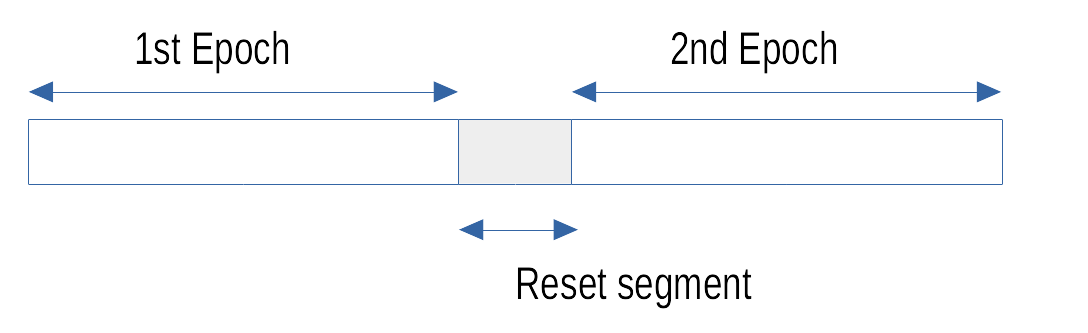
\includegraphics[width=0.8\textwidth]{img/epoch-concatenation}
  \caption{If the supervised learning is performed with different epoch of data, this is equivalent to a unique epoch, providing a reset segment of length $R$, the maximal recurrent range, is inserted before each new epoch. During reset segment, we set $\kappa_{nt}  = 0$.}
  \label{epoch-concatenation}
\end{figure}

\subsubsection*{Least-square adjustment} With respect to desired output $\bar{o}_n(t)$ we can write, in the ${\cal L}^2$ case:
\eqline{\rho_{nt}(\hat{x}_n(t)) = \frac{\kappa_{nt}}{2} (\hat{x}_n(t) - \bar{o}_n(t))^2}
On one hand, we choose $\kappa_{nt} > 0$ if $\bar{o}_n(t)$ is defined (output node) and $\kappa_{nt} = 0$ otherwise (hidden unit, missing data, or segmentation of the sequence in different epochs, while since $\kappa_{nt} \in [0, +\infty[$ it can also act as error gain, taking related precision into account. 

\subsubsection*{Robust criterion} One aspect of the estimation is related to robustness, i.e., being able to take into account the fact that errors and artifacts may occur in the learning set. It is implemented here as a M-estimator, i.e., not  a least-square function but another alternative cost function, with a smaller slope for higher values, as made explicit in Fig~\ref{robust-criteria}. This has been addressed, e.g, by \cite{ChenJain1994}.

With respect to usual M-estimators\footnote{For instance, for a bounded criterion a usual choice is the twice continuous differentiable biweight profile $\rho_{nt}(x) \equiv (x^6 - 3 \, x^4 + 3 \, x^2) \, H(1 - |x|) + H(|x| - 1)$, with a hard threshold at $x_{thres} = 1$.}, we propose here to use reweighted quadratic criterion, i.e., consider a previous estimation $\hat{\bf x}$ of ${\bf x}$, in order to locally work at each step with a least-square criterion, namely:
\[
  {}_1\rho_{nt}(x) \equiv \frac{x^2}{\nu + |\hat{x}|} \mbox{ or } {}_0\rho_{nt}(x) \equiv \frac{x^2}{\nu + \hat{x}^2},
\]
for unbounded and bounded profiles. This is equivalent to use an approximate criterion derivative.

For small values of $\nu$ the criterion allows to perform sparse estimations. Anyway, the value of $\nu$ is not to be adjusted manually, but can simply be set at a fraction of the criterion minimal value, say $\nu \simeq 10^{-3} \, \rho_{\min}$. 

\begin{figure}[!ht]
 \centerline{
  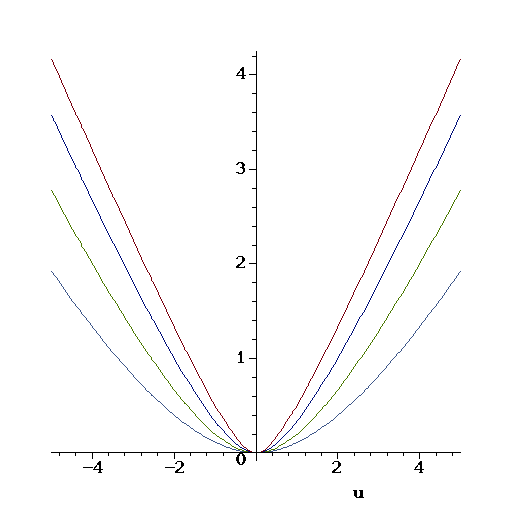
\includegraphics[width=0.4\textwidth]{img/m1-profile-1}
  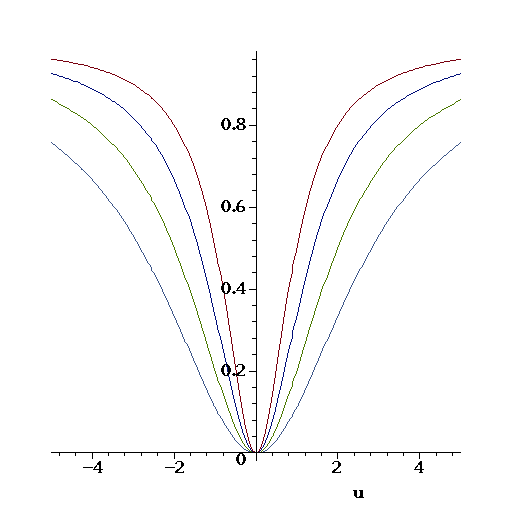
\includegraphics[width=0.4\textwidth]{img/m1-profile-2}
}
  \caption{Two examples of M1 profiles. Leftward, an unbounded profile, mollification of the ${\cal L}_1$ criterion, thus close to a ${\cal L}^2$ criterion for low values, and to a ${\cal L}^1$ criterion for high values: \centerline{$\rho_{nt}(x) \equiv \frac{x^2}{\nu + |x|} = x^2 / \nu + O(|x|^3) = |x| - \nu + O(1/|x|)$,} for $\nu = 1,2,4,8$. Rightward, a bounded profile, mollification of the ${\cal L}_0$ criterion: \centerline{$\rho_{nt}(x) \equiv \frac{x^2}{\nu + x^2} = x^2 / \nu + O(x^4) = 1 + O(1/x^2)$,} for $\nu = 1,2,4,8$.}
  \label{robust-criteria}
\end{figure}

\subsubsection*{Boolean adjustment} Another aspect of the estimation is the fact that we may have to estimate Boolean value, i.e., with the notations of this paper, requires the values $\hat{x}_n(t)$ to be lower or higher than $1/2$, according to $\bar{o}_n(t)$. Taking a margin $\nu$ into account, and considering a quadratic criterion, a natural choice writes:
\eqline{\rho_{nt}(\hat{x}_n(t)) = \frac{\kappa_{nt}}{2} q\left(\nu - sg(\bar{o}_n(t) - 1/2) \, (\hat{x}_n(t) - 1/2)\right), \;\;\; q(v) \deq H(v) \, v^2}
where $sg()$ is the sign function, which is a criterion that vanishes if and only if $|\hat{x}_n(t) - 1/2| > \nu$ and has the right sign, while it behaves as a quadratic criterion otherwise.

\subsubsection*{Stochastic adjustments} A step further, we may not be interested to perform a deterministic adjustment, but to optimize the output probabilistic distribution with respect to the desired output distributions, as e.g., in \cite{cofre:hal-00861397} for spiking neuron networks adjustment. As developed in appendix~\ref{stochastic}, the weight estimation problem can be related to the following criterion:
\eqline{\rho({\bf x}) \deq \sum_k |\lambda_k| \, \left|\bar{\Omega}_{k} - \frac{1}{T-\tau_k} \sum_t \omega_k(t)\right|,}
for some observable $\omega_k(t)$, with average value $\bar{\Omega}_{k}$, and parameters $\lambda_k$ made explicit in appendix~\ref{stochastic} and considered here as input.

We may for instance consider mean and auto-correlation as in appendix~\ref{stochastic}, or instantaneous momenta at time $t$, e.g., mean and variance, considering a Gaussian distribution.

\subsubsection*{Considering static estimation.}

The present framework stands for dynamic estimation of a temporal sequence. It can also simply be applied to a static estimation at the final time step $T-1$ considering $\bar{o}_n(T-1)$ only the previous values $o_n(t)$ being unconstrained. In that case the value $T$ corresponds to the number of iteration to obtain the desired estimation. In a non-recurrent architecture this value is easy to derive from the architecture, it corresponds to the number of computation steps. In a recurrent architecture, the situation is more complex since computation loops have to converged, and the number of computation steps is an explicit parameter, unless the system is tuned to converge to a fixed point, while considering $T \rightarrow +\infty$ which is a rather straightforward extension of the present work.

\subsection*{Considering constrained architecture and weights values.}

It is precious to also introduce constraints on the connection weights. Typical constraints include: 
\\- sparse connectivity, which reduces the total amount of computation, and allows internal sub-assemblies to emerge, 
\\- positive or negative weight values (corresponding to excitatory or inhibitory connections).

The design choice of the kernels allows us to constraint the network connectivity. It is possible to specify partial connectivity allowing to distinguish different layers (e.g. hidden layers not connected to input and/or output).
This may be, for instance, a 2D-topography with local horizontal connections, or several layers with, e.g., either point to point, or divergent connectivity between layers.

However, if the architecture itself has to be learned, the present framework may be used in another way: Starting from a given connected network and performing a sparse estimation, may lead to a result with zero weight values for connections not present in the estimated architecture, and non zero values otherwise. This is a sparse estimation, i.e. not only minimizing the metric not only with respect to the weights values, but also with respect to the fact that some weights have either zero or non-zero values, i,e, with respect connection sets. Sparse estimation methods (see e.g. \cite{tropp:04a,tropp:04b} for a didactic introduction) can be used to this end. 

One application could be modulatory weighted connections, allowing to enhance or cancel sub-parts of the network connectivity.

One track is to simply choose, for some meta-parameters $\nu_{nd}$: 
\eqline{{\cal R}({\bf W}) = \sum_{nd} \frac{\nu_{nd}}{\epsilon + |\hat{W}_{nd}|} \, W_{nd}^2}
where $\hat{W}_{nd}$ stands for the best a-priory or previous estimation of the weight. This leads to a reweighted least-square criterion, where small weights value minimization is reinforced, up to $0$, yielding sparse estimation.

The case where we consider excitatory or inhibitory connections (i.e., weight values that only positive or negative), or the case where the weights are bounded, is managed at the implementation level, as a hard constraint in the minimization. Very simply, if the value is beyond the bound it is reprojected on on the bound. This may lead to a sub-optimal estimation, but avoids the heavy management of Karush-Kuhn-Tucker conditions.

As an example, let us consider the adjustable leak $\gamma_{nt}$, $0 \leq \gamma_{nt} \leq 0.99 \simeq 1$ of a NLN unit. If the minimization process yields a negative value, the value is reset to zero (it means that we better have no leak). If the minimization process yields an unstable value higher than one, it is reset to, say, $0.99$ to be sure the system will not diverge.

\subsection*{Considering un-supervised regularization.}

In order to find an interesting solution, we have to constraint the hidden activity to be estimated. Interesting properties includes sparseness, orthogonality, robustness and bounds.

Sparse activity (i.e., with a maximal number of values closed or equal to zero), which is known to correspond to unit assemblies tuned to a given class of input statistics, can be specified as a reweighted least-square criterion again, for some meta-parameters $\kappa_{nd}$:
\eqline{\rho_{nt}(x_{nt}) = \frac{\kappa_{nd}}{\epsilon + |\hat{x}_{nt}|} \, x_{nt}^2}
where $\hat{x}_{nd}$ stands for the previous estimation, with an initial value equal to $\kappa_{nd}$, as previously discussed.

Orthogonality of hidden unit activities, in order to avoid redundancy and maximize the dynamic space dimension in the recurrent network, can also be specified, the same way as :
\eqline{\rho_{nt}(x_{nt}) = \kappa_{nd} \, \sum_{n' \neq n} (\sum_t x_{nt} \, \hat{x}_{n't})^2}
again as as, now not local but global, reweighted least-square criterion, now minimizing the dot products between unit activities, thus minimal when orthogonal. 

Another aspect concerns the fact we may have to control the activity bound, e.g., a weak constraint of the form $x_{nt} \preceq b$. Following the same heuristic, we may introduce a cost of the form:
\eqline{\rho_{nt}(x_{nt}) = \kappa_{nd} \, e^{k\,(x_{nt} - b)}}
with $k > 0$ in order to have a fast increasing function as soon as the bound is violated.
